% DO NOT COMPILE THIS FILE DIRECTLY!
% This is included by the other .tex files.

\begin{frame}[t,plain]
\titlepage
\end{frame}

\watermarkoff
\begin{frame}[t]{What is Mutt?}
\begin{itemize}
    \item Mutt is an email client - it lets you read your email.
    \item It does IMAP.
\end{itemize}
\end{frame}

\begin{frame}[t]{Why do I want Mutt}
\begin{itemize}
\item Because GUIs suck?
\item I want to use "insert editor here" to write my emails!
    \begin{enumerate}
        \item Ed - the standard editor!
        \item Vim
        \item Emacs
        \item Sublime
        \item Nano
        \item Anything else you can set \$EDITOR in bash to
    \end{enumerate}
\item Really good native PGP support.
\item Way more flexibility than traditional webmail.
    \begin{itemize}
        \item POP, imap, whatever the hell you want to run.
    \end{itemize}
\end{itemize}
\end{frame}

\begin{frame}[t]{Decomposing the "Checking your email" problem}
    \begin{itemize}
\item Webmail way: "I go to g.illinois.edu and then I log in to access my email, then I read my email, then I compose an email to someone else in the browser, and then I send it" (basically all-in-one approach from an end-user's perspective)
\item 1337 H@xx0r Way: "I use mpop/offlineimap to access my email, I use mutt/thunderbird to read my email, then I use msmtp to send my email"
\item Two different approaches, latter is more flexible in that you can swap components, but requires more work than former.
    \end{itemize}
\end{frame}

\begin{frame}[t]{Vocab}
\begin{figure}
    \centering
    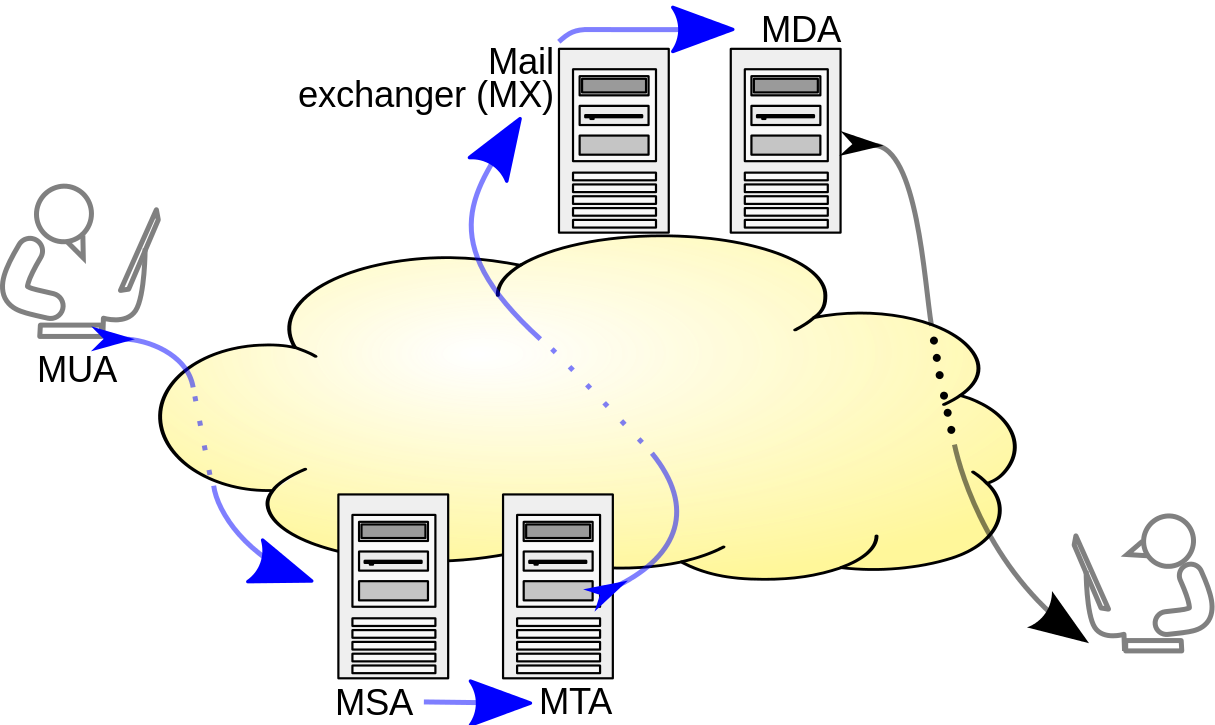
\includegraphics[width = 0.8\textwidth]{./SMTP-transfer-model.png}
    \caption[font=small]{STMP Transfer Model Illustrated. Now with 20\% more cloud!}
  \end{figure}
\end{frame}

\begin{frame}[t]{Vocab Cont.}
\begin{itemize}
    \item If you can get through this I will reward you with an adorable picture of a cat, and a Demo.
    \item Mail User Agent - read (Mutt)
    \item Mail Submission Agent - send to google's servers (msmtp or mutt)
    \item Mail Transfer Agent - Google's server, sends email (Postfix, Sendmail)
    \item Mail Exchanger - MX records? Load balancer to your MDA? Idk, never seen that terminology before.
    \item Mail Delivery Agent - Recieves email from the wider internet. (Postfix)
    \item POP3 Client - Downloads email from a server to your local computer (and deletes email off the server)
    \item IMAP Client - Synchronizes email from a server to your local computer
\end{itemize}
\end{frame}

\begin{frame}[t]{}
\begin{figure}
    \centering
    
\includegraphics[width = 0.8\textwidth]{./catComputer.jpg}
    \caption[font=small]{Mutt? No, I am a cat.}
  \end{figure}
\end{frame}

\begin{frame}[t]{Demo}
\begin{itemize}
    \item fetch: email command show zshrc
    \item read: show a little bit of what mutt looks like
    \item send: demonstrate sending an email
\end{itemize}
\end{frame}

\begin{frame}[t]{I want this! How can I haz setup!}
\begin{itemize}
    \item Mutt by itself has an imap client built in
        \begin{itemize}
            \item Simplest to configure.
            \item this means you can read your email, stored on google's servers without ever having actually downloaded the actual contents of the email.
            \item Slow.
            \item Can't read email on your laptop without internet.
        \end{itemize}
    \item Better solution: Use offlineimap or mpop or similar software to download emails to your local computer, store in plaintext on your local disk, and then point mutt at the copies on your local disk
        \begin{itemize}
            \item added features: You can grep, awk, vim, sed, your emails if you store them in plaintext
            \item if you use pop, the emails stay on your personal computer instead of a remote server, and LE has to get a warrant to get their hands on your communications instead of simply bullying google for them
            \end{itemize}
\end{itemize}
\end{frame}

\begin{frame}[t]{Install/Configuration}
\begin{itemize}
    \item Install through package manager.
    \item Google config walkthroughs.
    \item I will provide a walkthrough here, but these setups get pretty customized pretty fast
    \item \href{https://github.com/ACMLug/meetings/tree/master/meeting5-2014-10-06}{Configs on Github}
    \item That's all folks!
\end{itemize}
\end{frame}
